\section{Method}\label{method}

\begin{figure}
\centering
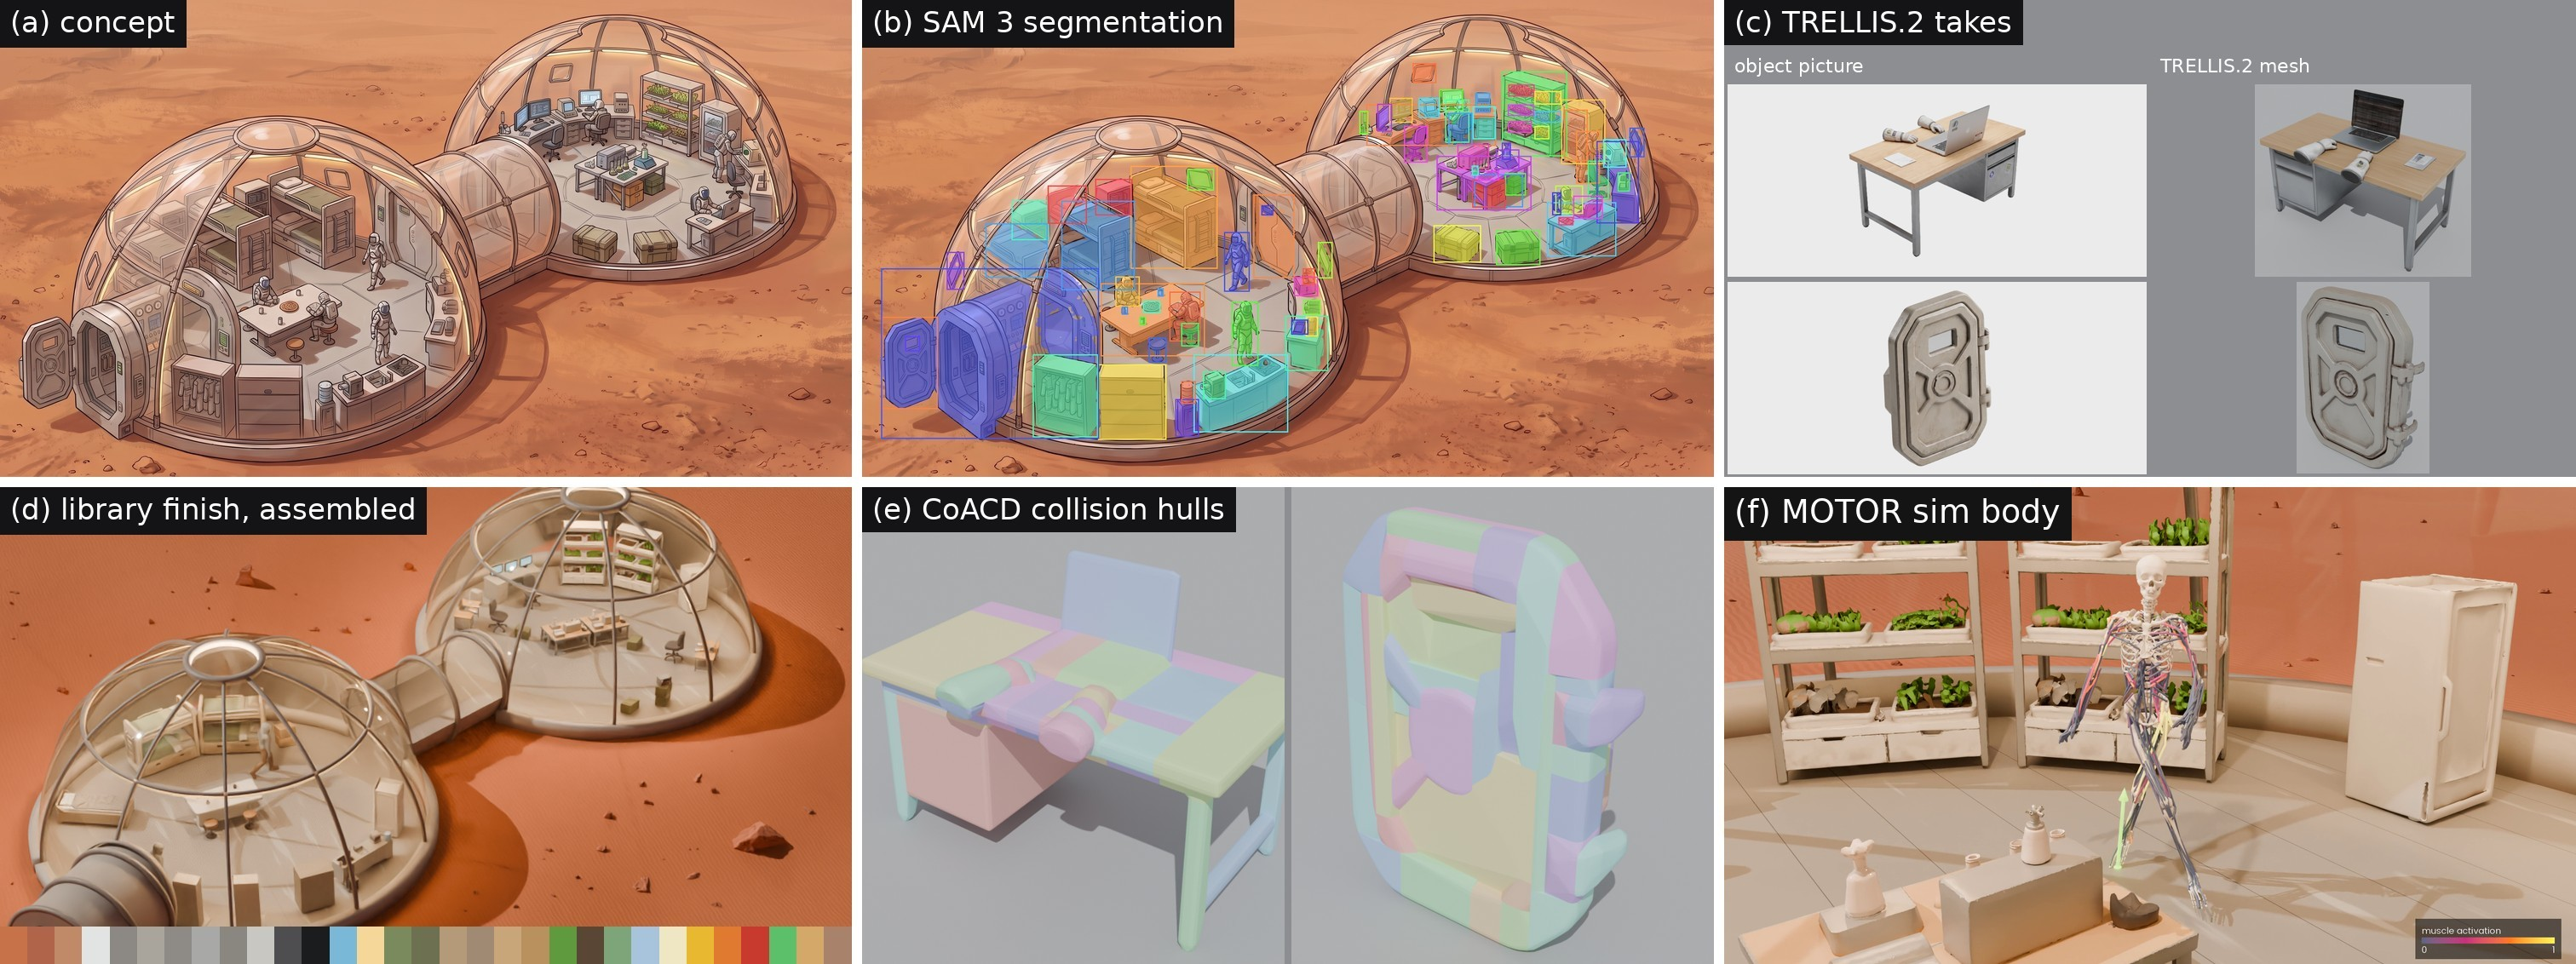
\includegraphics[width=1\linewidth,height=\textheight,keepaspectratio,alt={One place, camp, through SCORE's layers. (a) The creator's locked concept. (b) SAM 3 segments it into 80 instances from its probe nouns. (c) The two objects of camp made by TRELLIS.2, each close-up beside its generated mesh. (d) The assembled place, every surface finished from the place's library palette (strip, 31 tokens). (e) CoACD convex decomposition written with the model (43 hulls for the desk, 48 for the door), with mass, friction and restitution from the material class. (f) A walker's MyoFullBody sim body, solved by MOTOR, in the finished place.}]{figures/layers.jpg}
\caption{One place, camp, through SCORE's layers. (a) The creator's locked concept. (b) SAM 3 segments it into 80 instances from its probe nouns. (c) The two objects of camp made by TRELLIS.2, each close-up beside its generated mesh. (d) The assembled place, every surface finished from the place's library palette (strip, 31 tokens). (e) CoACD convex decomposition written with the model (43 hulls for the desk, 48 for the door), with mass, friction and restitution from the material class. (f) A walker's MyoFullBody sim body, solved by MOTOR, in the finished place.}
\end{figure}

SCORE records every scene as an OpenUSD stage, with its physics in UsdPhysics and each child scene held by reference, so that each of the layers below can be edited without disturbing the others. Before anything is drawn, the creator decides the physics, the setting and the style of the environment: its gravity and ground, where it lies, and a style line with reference pictures. An interview with Gemini 3.1 Pro \citep{gemini31pro} drafts this environment concept, and the creator locks it.

Each place then passes through the layers shown in Figure 1. Its concept picture is drawn by Nano Banana Pro through the Google Gemini API \citep{nanobananapro} from the place's contents, view and style, and the creator locks it in turn. SAM 3 \citep{carion2025sam3} segments the locked picture into an inventory of its objects. A coding agent \citep{claudecode} lays library pieces over that inventory in Blender \citep{blender}, renders the concept view and corrects the layout until it reads as the concept. Objects that the library does not hold are made by TRELLIS.2 \citep{xiang2025trellis2} from the concept's own crop of them and fitted in their place.

Generated objects arrive with colours of their own, which would make a scene look assembled from unrelated sources. The library finish therefore moves each generated colour towards the nearest colour of the place's single palette, and replaces any colour that stays far from it with a library surface \citep{raistrick2026procfunc}, so that made and library objects share one look. CoACD \citep{wei2022coacd} then gives every model convex colliders, with its mass and friction taken from its material.

The assembled scene is checked before it counts as ready. Twelve kinds of fault are tested, among them objects floating above their support, objects passing through one another and walkways too narrow to use, and in MuJoCo every loose object is released for one second; any object that slides or tips fails the scene.

Finally the place is populated. People are routed over the checked floor, animated by Kimodo \citep{rempe2026kimodo} along those routes as described below, and solved by MOTOR \citep{motor} as MyoFullBody sim bodies sized to their SOMA bodies \citep{saito2026soma}. MOTOR recovers the joint motion, computes the ground reaction forces from the contact of the skin with the floor and the joint moments under the place's gravity, and shares those moments over the 416 muscles. A body is accepted when its residual forces and moments stay within the limits of the residual check \citep{hicks2015verification}.

Each walker is routed over the same floor that the scene check reads. In the manner of Recast \citep{recast}, the scene's solids, shut doors included, are sampled on a 12.5 cm grid into walkable spans with 1.7 m of headroom, joined where the step between them is at most 30 cm and eroded from the walls so that a walkway 0.9 m wide remains; a stair flight is then simply a run of spans one riser apart. Dijkstra's algorithm \citep{dijkstra1959} finds the shortest route between the walker's spots, which is straightened, rounded at its corners and timed. Because Kimodo makes at most ten seconds of motion per request, the route is cut into walking and climbing pieces, each keyed to the pose that ends the previous one, and a door on the route swings open shortly before the walker reaches it (Figure 2).

\makeatletter\def\fps@figure{!t}\makeatother

\begin{figure}
\centering
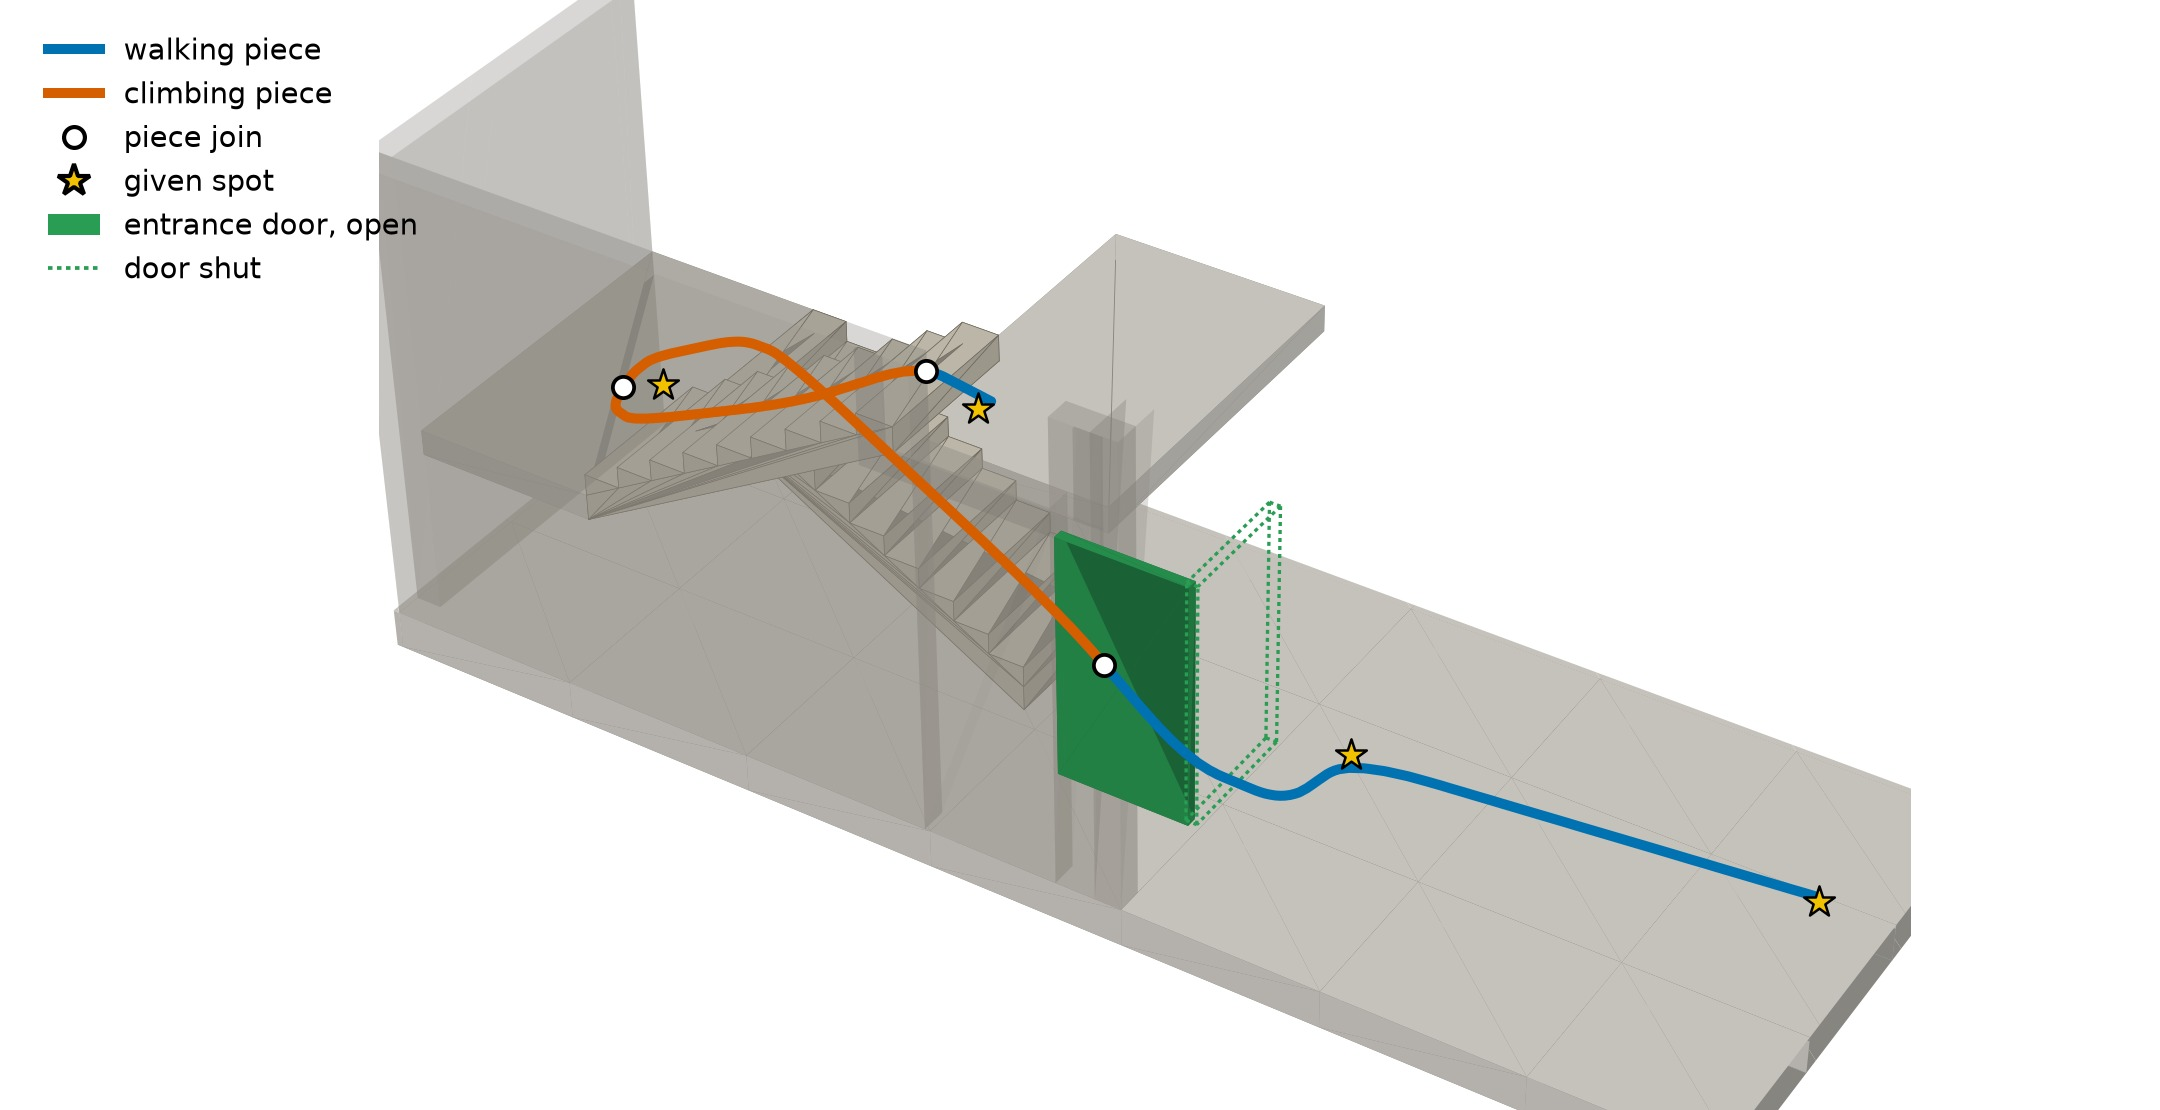
\includegraphics[width=1\linewidth,height=\textheight,keepaspectratio,alt={The woman's route through the stairwell, drawn in 3D over its stairs, landings and walls. The route is cut into walking and climbing pieces for Kimodo, each joined to the next at a circle, and passes through the given spots (stars). The entrance door is swung open from its shut position (dotted) shortly before she reaches it.}]{figures/route.jpg}
\caption{The woman's route through the stairwell, drawn in 3D over its stairs, landings and walls. The route is cut into walking and climbing pieces for Kimodo, each joined to the next at a circle, and passes through the given spots (stars). The entrance door is swung open from its shut position (dotted) shortly before she reaches it.}
\end{figure}
